\documentclass[a4paper,12pt]{article}
\usepackage[utf8]{inputenc}
\usepackage[spanish]{babel}
\usepackage{amsmath}
\usepackage{amsfonts}
\usepackage{amssymb}
\usepackage{multirow}
%\usepackage{makeidx}
\usepackage{graphicx}
\usepackage{fancyhdr}
\usepackage{hyperref}
\usepackage{float}
\usepackage{color}
\definecolor{azulUC3M}{RGB}{0,0,102}
\definecolor{gray97}{gray}{.97}
\definecolor{gray75}{gray}{.75}
\definecolor{gray45}{gray}{.45}
\usepackage{listings}
\lstset{ frame=Ltb,
     framerule=0pt,
     aboveskip=0.5cm,
     framextopmargin=3pt,
     framexbottommargin=3pt,
     framexleftmargin=0.4cm,
     framesep=0pt,
     rulesep=.4pt,
     backgroundcolor=\color{gray97},
     rulesepcolor=\color{black},
     %
     stringstyle=\ttfamily,
     showstringspaces = false,
     basicstyle=\small\ttfamily,
     commentstyle=\color{gray45},
     keywordstyle=\bfseries,
     %
     numbers=left,
     numbersep=15pt,
     numberstyle=\tiny,
     numberfirstline = false,
     breaklines=true,
   }
 
% minimizar fragmentado de listados
\lstnewenvironment{listing}[1][]
   {\lstset{#1}\pagebreak[0]}{\pagebreak[0]}
 
\lstdefinestyle{consola}
   {basicstyle=\scriptsize\bf\ttfamily,
    backgroundcolor=\color{gray75},
   }
 
\lstdefinestyle{C}
   {language=C,
   }
\usepackage[top=2cm]{geometry}
\pretolerance=2000
\tolerance=3000
\begin{document}

\begin{titlepage}
\begin{sffamily}
\color{azulUC3M}
\begin{center}
%\vspace*{-1cm}
\begin{figure}[htb]
\begin{center}
\vspace*{0.6cm}

\includegraphics[width=15cm]{imagenes/Portada_Logo.png}
\vspace*{1.6cm}
\end{center}
\end{figure}
\begin{LARGE}
Máster Universitario en Ciberseguridad \\%completar el nombre del grado
2017/2018 \\%indicar el curso académico
\vspace*{1cm}
\textsl{Trabajo Fin de Máster}\\
\end{LARGE}
\Huge{\textbf{OpenRansim}}\\ %Más significativo que el anterior
\vspace*{1cm}
\rule{80mm}{0.1mm}\\
\huge{Íñigo Serrano Salgado}\\ %Separar cada autor con \\ 
\vspace*{0.5cm}
\begin{Large}
Tutor\\
Juan Tapiador\\
Lugar y fecha de presentación prevista\\
\end{Large}
\end{center}
\vspace*{2cm}
\color{black}
\emph{Palabras clave:} Ransomware, simulation, security, malware, encryption. \\
\emph{Resumen:} En este documento, se va a presentar una herramienta de código abierto que sirve para comprobar la protección de un sistema informático frente a ataques de Ransomware.\\
%
\includegraphics{imagenes/creativecommons.png}\\
%\emph{[Incluir en el caso de interés en su publicación en el archivo abierto]}\\
%Esta obra se encuentra sujeta a la licencia Creative Commons \textbf{Reconocimiento - No Comercial - Sin Obra Derivada}

\end{sffamily}
\end{titlepage}

\pagestyle{fancy}
\fancyhead{} % Clear all header fields
\setlength\headheight{21.2pt}
\lhead{\hspace*{-0.3cm}\raisebox{-0.3\height}{
\includegraphics[scale=1]{imagenes/Interior_Logo.png}}}
\rhead{\color{azulUC3M} OpenRansim} %Poner encabezado

\renewcommand{\tablename}{\textbf{Tabla}} %para poner la palabra en mayusucula
\renewcommand{\figurename}{\textbf{Figura}} % para poner la palabra en mayuscula
\renewcommand{\listtablename}{Índice de tablas}

\newpage

\tableofcontents

\newpage

\listoffigures

%Para imagenes
%\begin{figure}[H]
%\centering
%\includegraphics[scale=0.8]{imagenes/*.png}
%\caption{}
%\end{figure}

\newpage



%Comenzar el trabajo
\begin{abstract}
Hoy en día, uno de los ataques más comunes y eficaces que existen en el mundo de Internet, es el llamado Ransomware. Este tipo de ataques empezó a surgir en 1989 con AIDS Trojan. El Ransomware, se basa en secuestrar los datos de un sistema informático y pedir un rescate por estos. Técnicamente no requiere grandes conocimientos de seguridad para desarrollar un ejecutable, aunque, es cierto, que muchos emplean exploits para la fase de propagación. Lo cual lo convierte en uno de los ataques más efectivos y que suele obtener sus objetivos.\\\\
Es, por este motivo, que se ha decidido llevar a cabo este Trabajo de Fin de Máster, con el objetivo de aportar facilidades, para poder así evitar una infección en nuestros equipos y la consecuente remuneración para poder acceder de nuevo a nuestros archivos.
\end{abstract}

\newpage

\section{Introducción}
Como en muchas facetas de la vida real, la posibilidad de ganar dinero de forma fácil y a costa de los demás, ha llegado ya al mundo Online, como no podía ser de otro modo.\\\\
Con el paso de los años, han ido apareciendo muchos ciberdelincuentes o, incluso, mafias que están actuando a través de Internet. El secuestro de información, el ciberespionaje, el tráfico de cualquier dato sensible o la venta de piezas de malware, son cada vez más habituales en los tiempos que corren. Debido a esta serie de factores, es de vital importancia que exista, a disposición del usuario una ayuda como la presentada en este ensayo.\\\\
\begin{figure}[H]
	\centering
	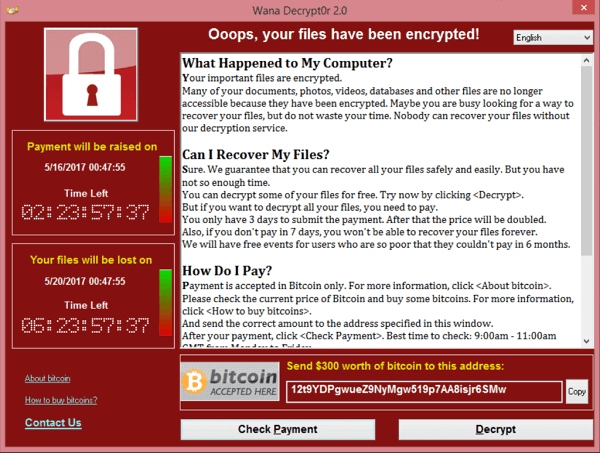
\includegraphics[scale=0.7]{imagenes/screenshot.png}
	\caption[Imagen que aparece en un ordenador infectado]{Imagen que aparece en un ordenador infectado}
	\label{fig:figure1}
\end{figure}
De todas las opciones que existen, los ataques de Ransomware, quizás sean los más rentables en términos económicos. Su único objetivo es secuestrar los datos de un ordenador para poder pedir un rescate por ellos. El uso de la criptografía y de las nuevas formas de pago, que garantizan el anonimato, son fundamentales para realizar un buen ataque.\\\\
El primer Ransomware que apareció, fue AIDS Trojan en 1989. Este malware escondía y cifraba los nombres de todos los ficheros que se encontrasen en el disco C. Esto hacia que el ordenador se quedase inservible, teniendo que pagar 189\$ a una oficina de correos en Panamá.\\\\
En 2011 apareció el primer Trojan, que se aprovechaba de la moda de los pagos anónimos como medio de pago del rescate de los datos. Actualmente, el uso de medios de pago anónimos es algo muy común, aunque no siempre es fácil para el atacante recuperar el dinero.\\\\
Según las últimas tendencias de Ransomware, el uso de criptografía simétrica es la forma más empleada para hacer que los datos no puedan recuperarse, a menos que se tenga la contraseña. Pero esto no siempre ha sido así, hubo un tiempo en el que la idea principal no era cifrar los datos de un ordenador, sino bloquearlo y hacer que su uso fuera limitado. Estos son los llamados "Lockers", que se valen de exploits y ciertas vulnerabilidades del sistema operativo anulando cualquier interacción con la máquina afectada.\\\\
Históricamente, este tipo de ataques ha estado siempre dirigido a ordenadores personales, por lo que los ordenadores con un sistema operativo de la familia Microsoft, eran más propensos a este tipo de ataque. Con la llegada de los Smartphone y la capacidad que tienen para ser ordenadores personales portátiles, en 2014 salió un Ransomware centrado en el sistema operativo Android.\\\\
El desarrollo del proyecto en cuestión, se centrará en la presentación de una nueva herramienta creada para facilitar la protección de sistemas informáticos frente a ataques de Ransomware. La idea en la que se basará este trabajo, surgió al descubrir algo similar en el mercado. Una aplicación llamada Ransim. Ésta, ejecuta una serie de escenarios, los más comunes, intentando asemejarse a un programa de Ransomware real.\\\\
El objetivo, es llevar a cabo los procedimientos necesarios para que, dicha herramienta, sea capaz de realizar la misma función que la previamente descubierta, aunque con una diferencia, y es que esta nueva herramienta presentaría un código abierto con posibilidad de ejecutar escenarios ad hoc. Por este motivo, el nombre elegido, ha sido OpenRansim. OpenRansim podrá encontrarse en la siguiente URL: \href{https://github.com/iserranos/OpenRansim}{Github}. 
Al tratarse de una aplicación de código abierto, cualquier persona con un cierto interés en el tema, podrá colaborar en su desarrollo, lo cual, será clave y podrá favorecer al correcto funcionamiento de la misma.
\subsection{Motivación del proyecto}
Parece ser, que nos encontramos en un nuevo mundo, el mundo de la digitalización. En este nuevo mundo, uno de los elementos más valiosos, ha pasado a ser la disposición de datos y su control. Por este motivo, el Ransomware, se ha convertido, en la opción con más posibilidades de hacer negocio para los ciberdelincuentes.\\\\
A comienzos del año 2017, apenas se conocía la existencia de este tipo de ataques, hasta que saltó a la fama WannaCry. En Mayo del mismo año, se lanzó un ataque masivo que afectó a nivel mundial, incluyendo grandes empresas españolas. El 27 de Junio de 2017 salió a la luz otro Ransomware llamado NotPetya. Este último también se propagó a escala mundial afectando a Ucrania, Estados Unidos e Italia, principalmente.\\\\
Debido al notable aumento de este tipo de ataques, la existencia de una herramienta que pueda medir, de forma fiable, como de protegido se encuentra un ordenador frente a este tipo de amenazas, pasa a convertirse en un recurso vital para compañías de todo el mundo. 
OpenRansim, ha sido desarrollado, para que cualquier persona, sea capaz de cubrir sus necesidades de protección ante posibles ataques de Ransomware. 
\subsection{Contribuciones}
Como todo proyecto final, es necesario que presente ciertas aportaciones, pudiendo ser mejoras de algo ya existente o totalmente nuevas en el sector. Para este proyecto se ha puesto el foco en presentar nuevas soluciones que ayuden, en la medida de lo posible, a que el mundo Online y de los ordenadores tenga más seguridad. Estas son las nuevas características que presenta OpenRansim: 
\begin{itemize}
	\item Simulador de Ransomware - Como aportación principal se encuentra OpenRansim, un simulador de Ransomware que verifica de forma rápida posibles infecciones sin afectar los datos del equipo.
	\item Modularidad - Este proyecto se ha desarrollado en módulos, haciendo que sea muy fácil de implementar nuevos snippets para los escenarios.
	\item Código abierto - El desarrollo de OpenRansim se ha hecho bajo la Licencia de código abierto GPL v3.0, permitiendo su uso a cualquier usuario, en cualquier ámbito y de forma gratuita.
	\item Fácil extensión - Gracias a la modularización de las operaciones más habituales, es muy sencillo reutilizar el código y crear un nuevo escenario sin necesidad de añadir nuevas funcionalidades.
	\item Optimización - Al estar implementado en Golang, permite un desarrollo muy rápido a la vez que un gran rendimiento, haciendo que se pueda ejecutar cualquier escenario en segundos, empleando los parámetros por defecto.
\end{itemize}
En la Sección 2 se introduce OpenRansim, cuales son sus funcionalidades y características. Posteriormente en la Sección 3 se describe cuales son las pruebas que se han realizado y los resultados obtenidos. En la Sección 4 se mencionan proyectos relacionados y las diferencias que tienen con éste. Finalmente, en la Sección 5 se concluye el trabajo y en los apéndices A y B se proporciona una descripción de la planificación y presupuesto del proyecto, respectivamente.
\newpage
\section{OpenRansim}
\subsection{Introducción}
OpenRansim es una herramienta de línea de comando, desarrollada en Golang bajo la licencia GPL 3.0 de uso libre. La puesta en marcha, se ha llevado a cabo, mediante la utilización de 10 escenarios básicos, aunque su diseño, basado en módulos, permite la creación de escenarios nuevos, haciendo que sea personalizable.
\begin{figure}[H]
	\centering
	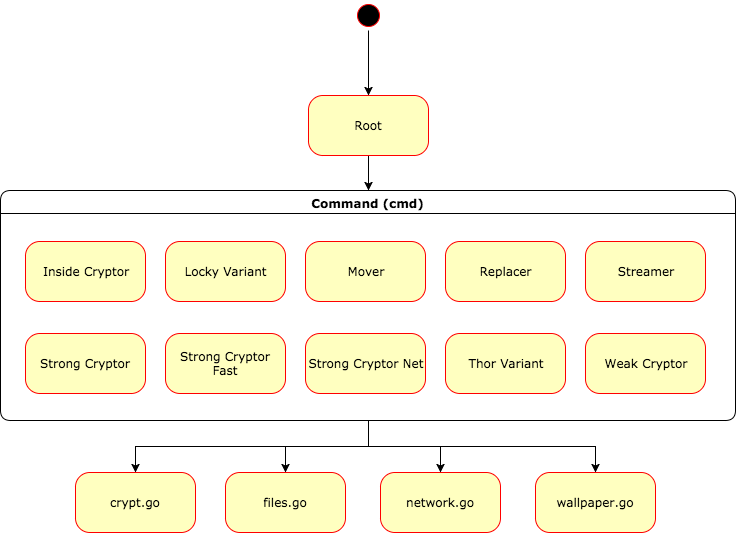
\includegraphics[scale=0.55]{imagenes/modules.png}
	\caption[Clases y módulos de OpenRansim]{Clases y módulos de OpenRansim}
	\label{fig:figure2}
\end{figure}
En la Figura ~\ref{fig:figure2} se muestra un diagrama de como está diseñado OpenRansim. En este programa se pueden apreciar tres bloques distintos: Root, Command y los ficheros externos de Golang.
\begin{itemize}
	\item Root - Este paquete representa el Framework empleado para crear CLI en Golang. Este es el punto de entrada de la herramienta y quien va a llamar a los diferentes comandos.
	\item Command - En este conjunto se encuentran los escenarios implementados. Estos, solo contienen el flujo de ejecución, pues la lógica se encuentra en el último grupo de clases. 
	\item Ficheros externos - Estos archivos ejecutable de Golang son los que contienen los métodos que, por ejemplo, crean directorios, listan ficheros, generan claves o hacen llamadas HTTP. 
\end{itemize}
\subsection{Pre task \& Post task}
Para comprobar que un escenario se ha ejecutado correctamente, y poder así dictaminar si existe una posibilidad de infección o no, se han añadido al desarrollo de la herramienta, las llamadas: pre-task y post-task. Antes de empezar a ejecutar un escenario, la herramienta crea una carpeta especifica donde se van a realizar las pruebas definidas por cada escenario. De esta forma se ejecuta la prueba bajo un entorno controlado sin que afecte a ningún archivo real.\\\\
Una vez ejecutado un escenario, es necesario comprobar si éste se ha completado correctamente o si, por el contrario, el sistema operativo ha interrumpido la ejecución, detectando y bloqueando, de esta manera, la posible acción maliciosa.  
\subsection{Escenarios}
Para esta primera versión de OpenRansim se han llevado a cabo una serie de escenarios, que intentan simular las ejecuciones de varios tipos de Ransomware. Para ello, se han estudiado cuales son las formas de funcionar de las familias de Ransomware más representativas. Estos son los 10 escenarios explicados obviando las fases de pre-task \& post-task: 
\begin{enumerate}
\item InsideCryptor – Cifra los datos y sobrescribe los archivos originales.
\begin{enumerate}
	\item Se va leyendo archivo por archivo. 
	\item Sobreescribe el mismo ficheros con los datos cifrados.
\end{enumerate}
\item LockyVariant – Simula una de las incontables variables del Ransomware Locky.
\begin{enumerate}
	\item Se va leyendo archivo por archivo.
	\item Crea un nuevo fichero con el mismo nombre y la extensión '.locky'
	\item Escribe los datos cifrados del ficheros original en el nuevo fichero.
	\item Elimina el fichero original.
\end{enumerate}
\item Mover – Cifra los datos en una carpeta diferente a la original y elimina los ficheros originales.
\begin{enumerate}
	\item Se va leyendo archivo por archivo.
	\item Crea un nuevo fichero con el mismo nombre pero en una carpeta distinta.
	\item Escribe los datos cifrados del ficheros original en el nuevo fichero.
	\item Elimina el fichero original.
	\item Elimina la carpeta original.
\end{enumerate}
\item Replacer – Reemplaza el contenido de los archivos.
\begin{enumerate}
	\item Escribe cadenas aleatorias en los ficheros. (No realiza ninguna operación criptológica).
\end{enumerate}
\item Streamer – Cifra todos los datos y los agrupa en un único fichero.
\begin{enumerate}
	\item Se va leyendo archivo por archivo.
	\item Cifra los datos de los ficheros y guarda el resultado en memoria.
	\item Cuando ha leido todos los ficheros crea uno en el que vuelca el contenido cifrado de todos los ficheros.
	\item Elimina todos los ficheros originales.
\end{enumerate}
\item StrongCryptor – Cifra los datos y borra los ficheros originales de forma segura.
\begin{enumerate}
	\item Se va leyendo archivo por archivo.
	\item Crea un nuevo fichero con el mismo nombre y la extensión '.copy'
	\item Escribe los datos cifrados del fichero original en su copia.
	\item Realiza 30 iteraciones escribiendo información cifrada aleatoria en el archivo original.
	\item Borra los archivos originales.
\end{enumerate}
\item StrongCryptorFast – Cifra los datos y borra los archivos originales.
\begin{enumerate}
	\item Se va leyendo archivo por archivo.
	\item Crea un nuevo fichero con el mismo nombre y la extensión '.copy'
	\item Escribe los datos cifrados del fichero original en su copia.
	\item Borra los ficheros originales.
\end{enumerate}
\item StrongCrytptorNet – Cifra los datos, borra los ficheros originales y simula una conexión HTTP.
\begin{enumerate}
	\item Se va leyendo archivo por archivo.
	\item Crea un nuevo fichero con el mismo nombre y la extensión '.copy'
	\item Escribe los datos cifrados del fichero original en su copia.
	\item Elimina los archivos originales.
	\item Realiza peticiones HTTP a un servidor mock con parte de la información cifrada.
\end{enumerate}
\item ThorVariant – Simula una de las incontables variables del Ransomware Thor.
\begin{enumerate}
	\item Se va leyendo archivo por archivo.
	\item Crea un nuevo fichero con el mismo nombre y la extensión '.thor'
	\item Escribe los datos cifrados del fichero original en su copia.
	\item Borra el archivo original.
	\item Cambia el wallpaper del ordenador.
\end{enumerate}
\item WeakCryptor – Utiliza un cifrado débil para cifrar los datos y elimina los archivos originales.
\begin{enumerate}
	\item Se va leyendo archivo por archivo.
	\item Crea un nuevo fichero con el mismo nombre y la extensión '.copy'
	\item Escribe los datos cifrados del fichero original en su copia.
	\item Borra los archivos originales.
\end{enumerate}
\end{enumerate} 
\subsection{Implementación}
Para el desarrollo de OpenRansim se ha utilizado el lenguaje Golang. Éste, desarrollado por Google, tiene las ventajas de C en tiempo de ejecución y las de Python, en velocidad de desarrollo. Para poder crear un CLI (Command Line Interface) se ha usado el Framework Cobra. Gracias a Cobra es muy fácil e intuitivo crear CLIs totalmente personalizables con comandos y flags de cualquier tipo. Como se observó en la Figura ~\ref{fig:figure2} la arquitectura de OpenRansim se divide en tres bloques. Los dos más importantes son el paquete cmd y el conjunto de ficheros externos.\\\\
El bloque cmd contiene todos los comandos que se pueden ejecutar. Estos comandos siguen una forma de implementarse definida por Cobra. Es por eso, que cada comando tiene una fase preliminar y otra posterior a la lógica propia del comando. Estos solo definen una serie de llamadas a funciones con diferentes parámetros de entrada para que se pueda crear un nuevo escenarios. Estas funciones se encuentran implementadas en el grupo de ficheros externos.\\\\
Estos, que actúan como librerías, contienen funciones muy genéricas y totalmente reutilizables que permiten crear flujos y escenarios muy variados. Dentro de estos ficheros encontramos los siguientes:
\begin{itemize}
	\item crypt - Dentro de esta libreria se pueden encontrar un conjunto de operaciones relacionadas con criptografía, es por eso que se usa una librería especial para generar números aleatorios. En este fichero tenemos las siguientes funciones:
	\begin{itemize}
		\item Cifrar - Esta función recibe como argumentos un texto en plano, una clave y un algoritmo de cifrado, a día de hoy solo se usan DES y AES. Devuelve un texto cifrado.
		\item Descifrar - Esta función tiene la misma firma que la anterior pero devolviendo texto en plano.
		\item Generar clave RSA - Esta función genera un par de claves RSA de las cuales se extrae la clave que se usará en cada escenario, si procede, para cifrar los archivos.
		\item Generar números aleatorios - Ya el propio nombre de la función explica su lógica. Se puede usar para rellenar ficheros, para poner nombres aleatorios o para la función anterior.
	\end{itemize}
	\item files - En esta clase se encuentran todas las funciones relacionadas con el tratamiento de ficheros.
	\begin{itemize}
		\item Crear directorio - Crea una carpeta en la ruta que se le pase por argumento.
		\item Comprobar que existe un directorio - Comprueba la existencia de una carpeta en la ruta que se le pase por argumento.
		\item Crear ficheros - Crea N ficheros en la carpeta seleccionada siempre y cuando se tengan permisos.
		\item Crear cadenas aleatorias - Genera N caracteres aleatorios que luego se concatena.
		\item Obtener información de ficheros - Obtiene toda la información relacionada con los archivos de una carpeta.
		\item Escribir en fichero - Escribe texto en un fichero.
		\item Leer de fichero - Devuelve todo el contenido de un fichero o un error.
		\item Eliminar fichero - Borra de forma permanente un archivo.
		\item Eliminar directorio - Elimina una carpeta y todos los ficheros que tuviera dicha carpeta.
	\end{itemize}
	\item network - Este fichero solo contiene la función de realizar peticiones HTTP. 
	\item wallpaper - Pasándole como parámetro una URL, cambia el fondo de pantalla por la imagen que se encuentra en esa URL.
\end{itemize} 
\subsection{BYOS, Build Your Own Scenario}
Debido a su gran modularidad, OpenRansim está diseñado para que pueda ser fácilmente extendido y/o mejorado. Cuando se habla de crear un nuevo escenario, es necesario saber un par de características de la herramienta que hacen que sea muy sencillo.\\\\
Como ya se ha comentado anteriormente, un escenario se basa en ejecutar las funciones que ya existen con los argumentos adecuados. Por lo que para construir un nuevo flujo, es posible que eligiendo las funciones adecuadas y el orden deseado se pueda crear un nuevo test. En caso de que las funciones ya existentes no sean suficientes, es posible crear unas nuevas en los ficheros ya existentes o nuevos ficheros. Gracias al diseño de OpenRansim, cualquier código que se añada a los ficheros externos o librerías van a estar disponibles para ser usadas en cualquier comando, sin necesidad de realizar nuevas importaciones ni precargas.
\newpage
\section{Validación experimental}
En esta sección se van a tratar varios puntos relacionados con el tiempo de ejecución y con los resultados de los diferentes escenarios.\\\\
\newpage
\section{Trabajos relacionados}
\newpage
\section{Conclusión}
No siempre se devuelven los archivos después de pagar
\appendix
\section{Planificación del proyecto}
\section{Presupuesto}

\end{document}
